Completa la Tabla \ref{tab:perimetro_lado} que muestra cómo cambia el perímetro de un cuadro
al variar la longitud de su lado.

\begin{table}[H]
    \centering
    \caption{Datos sobre la medida de los lados en un cuadrado con respecto al perímetro.}
    \label{tab:perimetro_lado}
    \begin{tabular}{|>{\columncolor{colorrds!80}\color{white}\bfseries}c|c|c|c|c|}
        \toprule
        Lado (cm)      & 0.5                 & 1                   & 2 & $\frac{5}{2}$        \\\cline{2-5}\midrule
        Perímetro (cm) & \ifprintanswers2\fi & \ifprintanswers4\fi & 8 & \ifprintanswers10\fi \\\cline{2-5}
        \bottomrule
    \end{tabular}
\end{table}

\begin{parts}
    \begin{minipage}{0.4\textwidth}
        \part ¿Cuál es el valor de la constante de proporcionalidad?

        \begin{solutionbox}{1.2cm}
            4
        \end{solutionbox}

        \part ¿Cuánto mide el lado de un cuadrado cuyo perímetro es cero?

        \begin{solutionbox}{1.2cm}
            0
        \end{solutionbox}

        \part ¿Cómo es el perímetro de un cuadrado que por lado mide 4 cm con respecto a otro cuadrado cuya longitud por lado es de 2 cm?

        \begin{solutionbox}{1.2cm}
            Es el doble.
        \end{solutionbox}
    \end{minipage}\hfill
    \begin{minipage}{0.4\textwidth}
        \part ¿Cómo se relaciona el perímetro de un cuadrado que por lado mide 4 cm con otro que mide 12 cm por lado?

        \begin{solutionbox}{1.2cm}
            Es la tercera parte.
        \end{solutionbox}

        \part ¿Cómo es la relación entre el perímetro de un cuadrado y la medida de uno de sus lados?

        \begin{solutionbox}{1.6cm}
            El perímetro de un cuadrado es cuatro veces la medida de una de sus lados.    \end{solutionbox}

        \part ¿Cuánto mide el lado de un cuadrado cuyo perímetro es de 1 cm?

        \begin{solutionbox}{1.2cm}
            0.25 cm.
        \end{solutionbox}

    \end{minipage}

    \part ¿Cuál de las gráficas representa la relación entre la longitud por lado y el perímetro de un cuadrado?

    \begin{figure}[H]
        \centering
        \ifprintanswers
            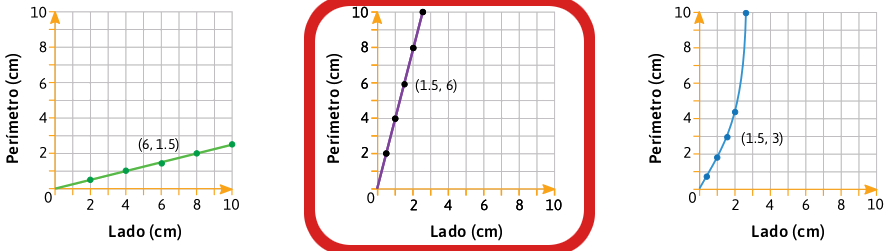
\includegraphics[width=0.9\linewidth]{../images/q70a_sol}
        \else
            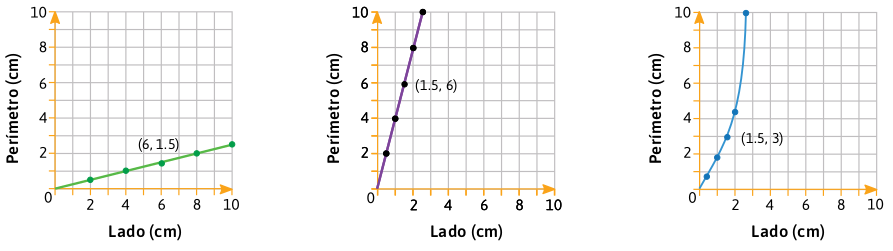
\includegraphics[width=0.9\linewidth]{../images/q70a}
        \fi
        \caption{}
        \label{fig:q70a}
    \end{figure}

    \part La gráfica que representa cómo cambia el perímetro con respecto a la longitud de su lado es creciente. ¿Por qué creen que recibe ese nombre?

    \begin{solutionbox}{1.6cm}
        Porque a cada aumento en la longitud del lado del cuadrado le co-
        rresponde un aumento en la longitud de su perímetro.
    \end{solutionbox}
\end{parts}